\documentclass{beamer}
\usepackage[utf8]{luainputenc}
\usepackage[french]{babel}
\usepackage{tikz}

\usetikzlibrary{matrix,chains,positioning,decorations.pathreplacing,arrows}
\setbeamertemplate{caption}[plain]{}

\usetheme{Luebeck}
\usecolortheme{seagull}

% Portion honteusement prise à `https://tex.stackexchange.com/questions/59893/page-counter-with-luebeck-theme`, pour afficher le nombre de diapositives
\setbeamertemplate{footline}
{%
  \leavevmode%
  \hbox{\begin{beamercolorbox}[wd=.1\paperwidth,ht=2.5ex,dp=1.125ex,leftskip=.3cm,rightskip=.2cm plus1fill]{author in head/foot}%
    \usebeamerfont{author in head/foot} \insertframenumber{} / \inserttotalframenumber
  \end{beamercolorbox}%
  \begin{beamercolorbox}[wd=.4\paperwidth,ht=2.5ex,dp=1.125ex,leftskip=.3cm plus1fill,rightskip=.3cm]{author in head/foot}%
    \usebeamerfont{author in head/foot}\insertshortauthor
  \end{beamercolorbox}%
  \begin{beamercolorbox}[wd=.5\paperwidth,ht=2.5ex,dp=1.125ex,leftskip=.3cm,rightskip=.3cm plus1fil]{title in head/foot}%
    \usebeamerfont{title in head/foot}\insertshorttitle
  \end{beamercolorbox}}%
  \vskip0pt%
}

\title[Reconnaissance d'espèces sous-marines]{Utilisation de l'apprentissage profond dans la reconnaissance d'espèces sous-marines}
\subtitle{TIPE -- MPSI 2018-2019}
\institute{Lycée F.D. Roosevelt, Reims}
\author{Lucas TABARY}
\date{12 juin 2019}

\begin{document}
  \maketitle
  \begin{frame}
    \frametitle{Sommaire}
    \tableofcontents
  \end{frame}

  \section{Principes élémentaires de fonctionnement d'un réseau neuronal}
  \subsection{Éléments structurants}
  \begin{frame}
    \frametitle{Neurone, poids et biais}

      \begin{tikzpicture}[
      init/.style={
        draw,
        circle,
        inner sep=2pt,
        font=\Huge,
        join = by -latex
      },
      squa/.style={
        draw,
        inner sep=2pt,
        font=\Large,
        join = by -latex
      },
      start chain=2,node distance=13mm
      ]
      \node[on chain=2]
        (x2) {$x_2$};
      \node[on chain=2,join=by o-latex]
        {$w_2$};
      \node[on chain=2,init] (sigma)
        {$\displaystyle\Sigma$};
      \node[on chain=2,squa,label=above:{\parbox{2cm}{\centering Fonction \\ d'activation}}]
        {$\sigma$};
      \node[on chain=2,label=above:Sortie,join=by -latex]
        {$y$};
      \begin{scope}[start chain=1]
      \node[on chain=1] at (0,1.5cm)
        (x1) {$x_1$};
      \node[on chain=1,join=by o-latex]
        (w1) {$w_1$};
      \end{scope}
      \begin{scope}[start chain=3]
      \node[on chain=3] at (0,-1.5cm)
        (x3) {$x_3$};
      \node[on chain=3,label=below:Poids,join=by o-latex]
        (w3) {$w_3$};
      \end{scope}
      \node[label=above:\parbox{2cm}{\centering Biais \\ $b$}] at (sigma|-w1) (b) {};

      \draw[-latex] (w1) -- (sigma);
      \draw[-latex] (w3) -- (sigma);
      \draw[o-latex] (b) -- (sigma);

      \draw[decorate,decoration={brace,mirror}] (x1.north west) -- node[left=10pt] {Entrées} (x3.south west);
      % Crédits : Gonzalo Medina, https://tex.stackexchange.com/questions/132444/diagram-of-an-artificial-neural-network
    \end{tikzpicture}

  \end{frame}
  \begin{frame}
    \frametitle{Fonctionnement général}
    \begin{figure}
      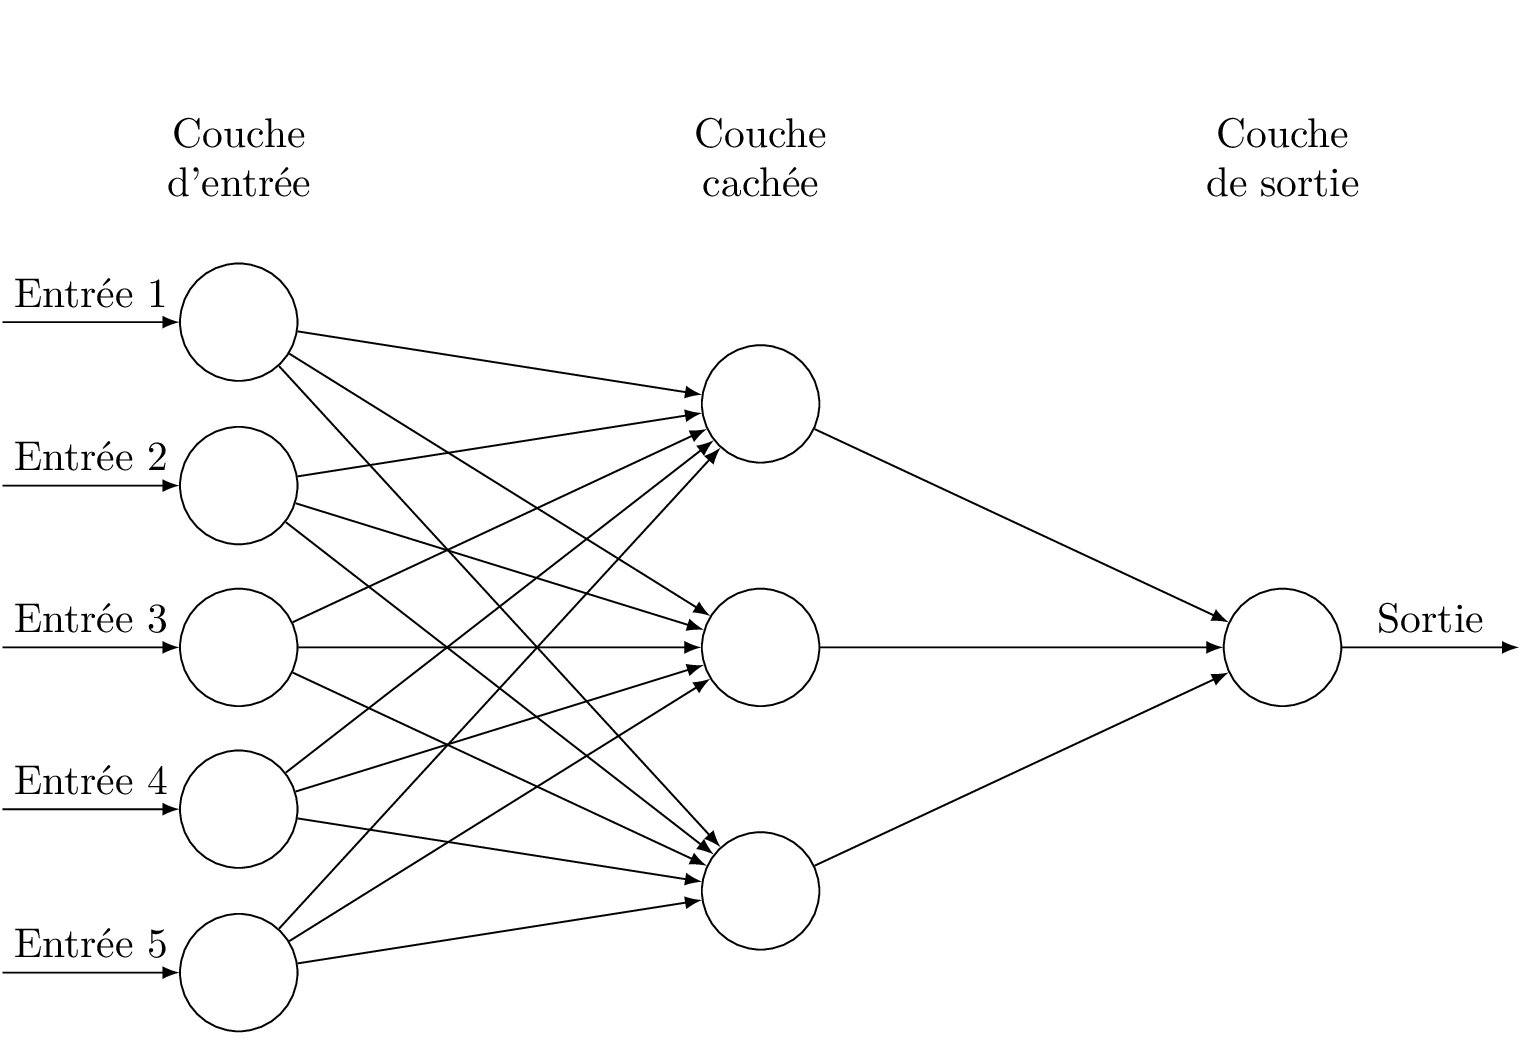
\includegraphics[scale=0.19]{Ressources/arbre.png}
    \end{figure}
  \end{frame}
  % \begin{frame}
  %   \frametitle{Formalisation}
  %   \begin{center}
  %     \begin{tabular}{lr}
  %       $w_{ij}^{(n)}$ & Poids du neurone $j$ (sur $n-1$) au neurone $i$ ($n$)\\
  %       $b_{i}^{(n)}$ & biais du neurone $i$ \\
  %       $a_i^{(n)}$ & activation du neurone $i$
  %     \end{tabular}
  %   \end{center}
  %     En choisissant $W^{(n)} = (w_{ij})$, $A^{(n)} = \left(a^{(n)}_i\right)$ et $B = (b_i)$, il vient
  %     \[
  %       A^{(n)} = \sigma\left(W^{(n)}A^{(n-1)} + B\right)
  %     \]
  % \end{frame}

  \subsection{Apprentissage du réseau}
  \begin{frame}
    \frametitle{Comment le réseau apprend-il~?}
      \begin{columns}
        \begin{column}{\dimexpr\linewidth-3cm-5mm}
          \[
            S(\lambda) = \left(w^{(1)}_{11}, w^{(1)}_{12}, \dots, w^{(n)}_{ij}, b^{(n)}_{j}\right) \quad\text{à l'étape $\lambda$}
          \]
          \[
            % P(T) = \sum_i \left(a_{i_{\text{attente}}} - a_{i_{\text{résultat}}}\right)^2
            C(S(\lambda))
            = \sum_{j} \left(a_{j_{\text{attente}}} - a_{j_{\text{résultat}}}\right)^2
          \]
          \[
            \vec\nabla C = \left(\frac{\partial C}{\partial w_{11}^{(1)}}, \frac{\partial C}{\partial w_{12}^{(1)}}, \dots, \frac{\partial C}{\partial b_{j}^{(n)}}\right)
          \]
          \[
            S(\lambda + 1) = S(\lambda) - \gamma\vec\nabla C
          \]
        \end{column}
        \begin{column}{5cm}
            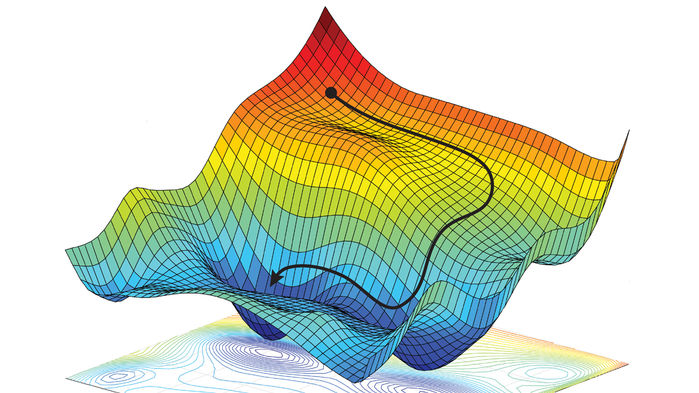
\includegraphics[width=5cm]{Ressources/gradient_descent.jpg}
        \end{column}
      \end{columns}
  \end{frame}

  \section{Modèles et utilisation}
  \subsection{Perceptron multicouche}
  \begin{frame}
    \frametitle{Perceptron multicouche}
    \begin{columns}
      \begin{column}{5cm}
        \begin{itemize}
          \item Conception élémentaire (ancienne, années 70)
          \item Détermination simple des dérivées partielles
        \end{itemize}
        \[
          \frac{\partial C}{\partial w^{(2)}_{11}} = \underbrace{\frac{\partial C}{\partial a^{(2)}_{1}}}_{\text{connu}} \times \frac{\partial a^{(2)}_{1}}{\partial w^{(2)}_{11}}
        \]
        \[
          a^{(2)}_{1} = \sigma\left(C + w^{(2)}_{11}a^{(1)}_1 + b^{(2)}_1\right)
        \]
        \[
          \frac{\partial a^{(2)}_{1}}{\partial w^{(2)}_{11}} = a^{(1)}_1 \times \sigma'\left(C + w^{(2)}_{11}a^{(1)}_1 + b^{(2)}_1\right)
        \]
      \end{column}
      \begin{column}{5cm}
        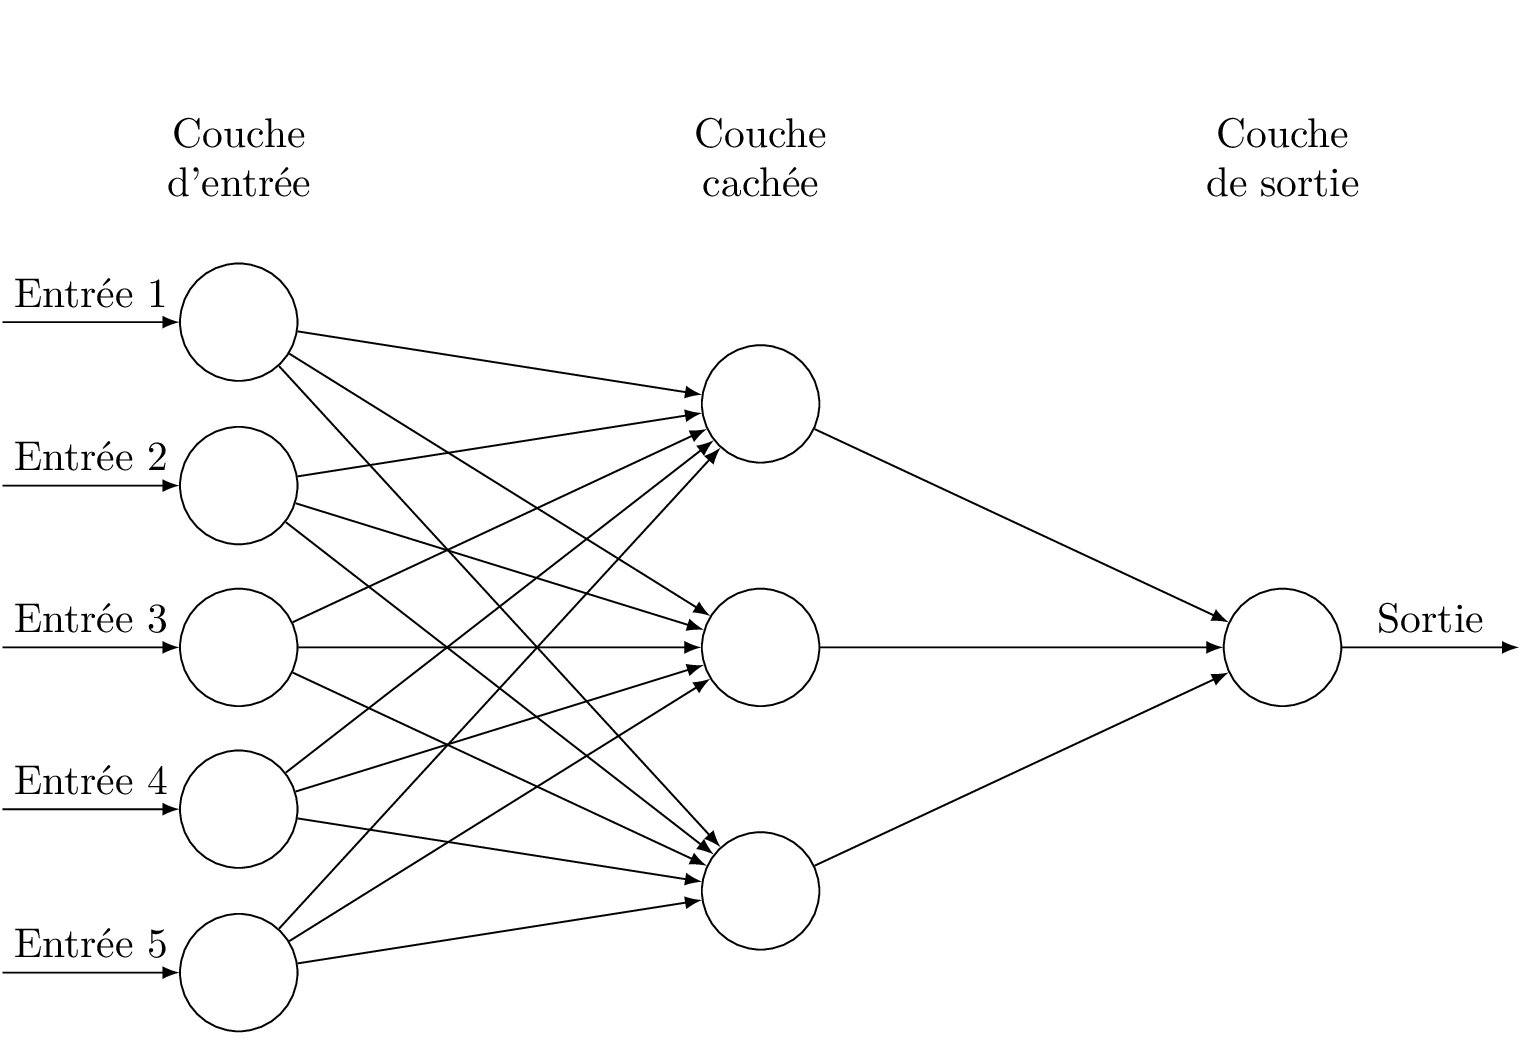
\includegraphics[width=5cm]{Ressources/arbre.png}
      \end{column}
    \end{columns}
  \end{frame}

  \subsection{Réseau de neurones convolutifs}
  \begin{frame}
    \frametitle{Spécificités d'un \textit{CNN}}
    \begin{figure}
      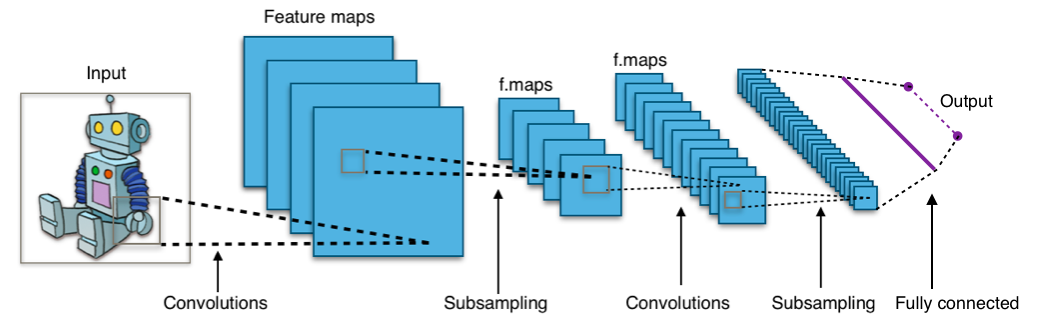
\includegraphics[scale=0.29]{Ressources/CNN.png}
    \end{figure}
    \begin{itemize}
      \item Couche de convolution~: produit de convolution~;
      \item Couche de mise en commun \textit{pooling}~: \textit{max pooling}, \textit{average pooling}.
    \end{itemize}
  \end{frame}
  \subsection{Cas réel d'étude}
  \begin{frame}
    \frametitle{Préparation du modèle pour correspondre à l'étude}
    \begin{itemize}
      \item Utilisation de \textit{TensorFlow}
      \item Nécessité d'un ensemble de données suffisant (\textit{Fish4Science})
      \begin{itemize}
        \item Traitement préalable
        \item Formatage pour le réseau
      \end{itemize}
    \end{itemize}
    \begin{columns}
      \begin{column}{0.3\textwidth}
        \tiny\begin{tabular}{|c|} \hline
          32 matrices $5\times5$ de convolution \\ \hline
          \textit{Max pooling} $3\times3$ \\ \hline
          64 matrices $3\times3$ de convolution \\ \hline
          \textit{Max pooling} $2\times2$ \\ \hline
          64 matrices $3\times3$ de convolution \\ \hline
          Couche dense (100) \\ \hline
          Couche dense (64) \\ \hline
          Couche dense de sortie (23) \\ \hline
        \end{tabular}
      \end{column}
      \begin{column}{0.7\textwidth}
        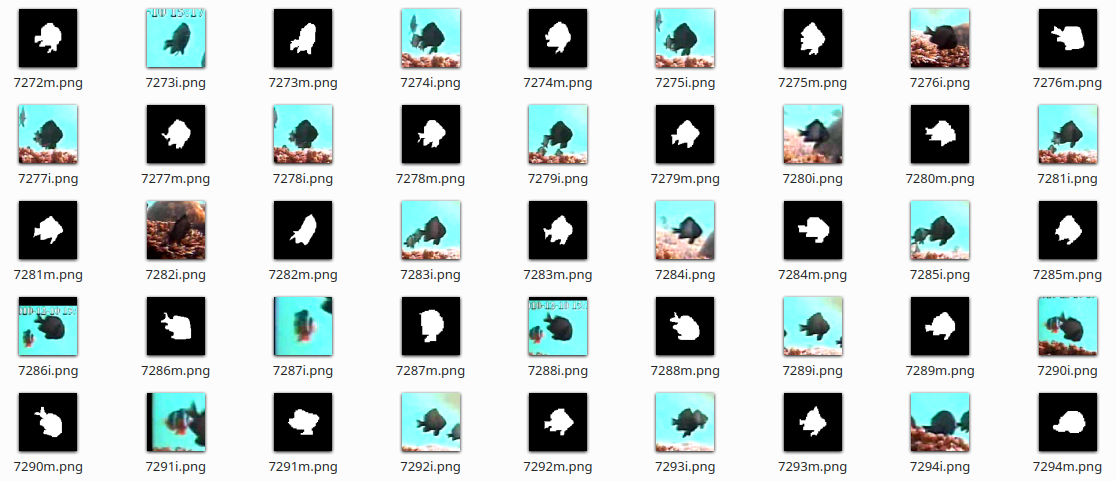
\includegraphics[scale=0.25]{Ressources/DB.png}
      \end{column}
    \end{columns}
  \end{frame}

  \section{Résultats et analyses}
  \subsection{Présentation des résultats}
  \begin{figure}
    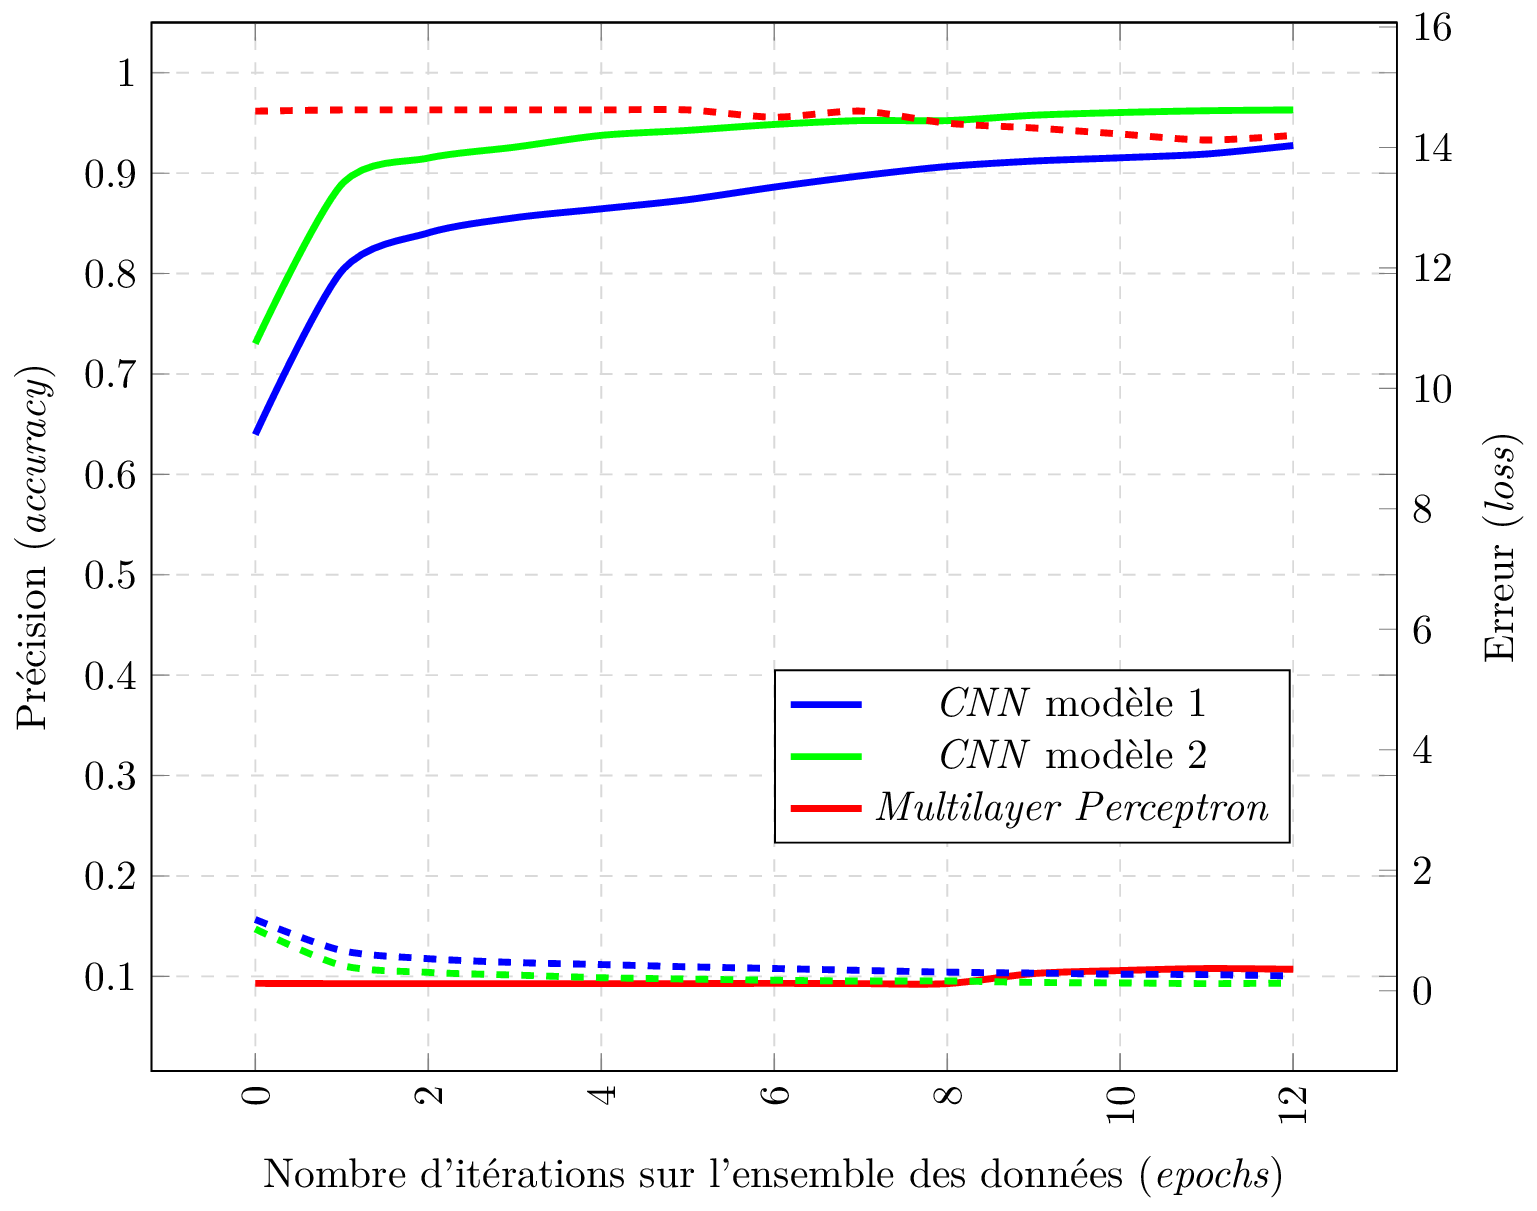
\includegraphics[scale=0.19]{Ressources/graph.png}
  \end{figure}
  \begin{frame}
    \nocite{3B1B:2018, Branson:2014, Rathi:2018, Rojas:1996, TF}
    \bibliographystyle{siam}
    {\fontfamily{lmr}\selectfont
      \bibliography{../references.bib}
    }
  \end{frame}









\end{document}
